\documentclass[xcolor=table,dvipsnames,table]{beamer}
\mode<presentation>
\usetheme{boxes}
\setbeamertemplate{navigation symbols}{}
% http://www.latex-community.org/forum/viewtopic.php?f=4&t=6694
\setbeamertemplate{navigation symbols}{\raisebox{5pt}{\makebox[\paperwidth]{\hfill\makebox[10pt]{\scriptsize\insertframenumber\vspace{1ex}}}}}
%\setbeamertemplate{footline}[frame number]
\setbeamertemplate{blocks}[shadow=false]
%\setbeamercolor*{block title}{fg=structure,bg=RoyalBlue!10}
\setbeamercolor*{block title example}{fg=structure,bg=RoyalBlue!10}
%\setbeamercolor*{block title example}{fg=BrickRed,bg=Goldenrod!10}
\setbeamercolor*{block title alerted}{fg=white,bg=black}
\addtobeamertemplate{block begin}{\pgfsetfillopacity{0.8}}{\pgfsetfillopacity{1}}
%\rowcolors{0}{RoyalBlue!20}{RoyalBlue!5}
\setbeamertemplate{caption}{\raggedright\insertcaption\par}

%\DeclareGraphicsRule{*}{mps}{*}{}

\usepackage{latexsym}
\usepackage{hyperref}
\usepackage{tikz}
\usetikzlibrary{calc,shapes,arrows,shadows,shapes.callouts,shapes.arrows,chains,positioning,trees}
\usepackage{solution}
\usepackage{calc}
\usepackage{pifont}
\usepackage{algorithmic}
\usepackage{pdfcomment}
\usepackage{color}

\newcommand{\cmark}{\ding{51}}
\newcommand{\xmark}{\ding{55}}

\newcommand{\highlight}[1]{{\color{blue}{#1}}}
\newcommand{\mycite}[1]{{\color{darkgray}{\footnotesize [#1]}}}

\DeclareMathOperator*{\argmin}{arg\,min}
\DeclareMathOperator*{\argmax}{arg\,max}
\DeclareMathOperator{\sign}{sign}
\DeclareMathOperator{\cnt}{Count}

\newcounter{mycallout}

\newcommand{\callouts}[3]{%
  \stepcounter{mycallout}
  \tikz[remember picture,baseline]{\node[anchor=base,inner sep=0,outer sep=0]%
    (\themycallout) {\colorbox{#1!20}{#3}};\pause\node[overlay,rectangle callout,%
    callout relative pointer={(0cm,0.5cm)},fill=#1!20] at ($(\themycallout.south)+(-0cm,-0.7cm)$){#2};}%
    }%

\raggedright

\newcount\lecturecount
\lecturecount=0
\AtBeginLecture{%
    \advance\lecturecount by 1
    \date{}
    \begin{frame}
    \begin{center}
    \titlepage
    \ifnum\lecturecount=1
    Part \the\lecturecount: \insertlecture
    \else
    Part \the\lecturecount: \insertlecture
    \fi
    \end{center}
    \end{frame}
}

\addtobeamertemplate{block begin}{\setlength\abovedisplayskip{0pt}}

%\newcommand{\example}[1]{{\color{BrickRed!50}{#1}}}
\newcommand{\maths}[1]{{\color{RoyalBlue!50}{#1}}}
\newcommand{\reference}[1]{{\color{RoyalBlue!30}\tiny [from #1]}}
\newcommand{\koehnref}{\reference{\href{http://www.statmt.org/book}{P.Koehn SMT book slides}}}


\ifx\pdfoutput\undefined
  \usepackage{graphicx}
\else
  %\usepackage[pdftex]{graphicx}
  \DeclareGraphicsRule{*}{mps}{*}{}
\fi
\newcommand{\argmax}[1]{\begin{array}{c}\mbox{arg max}\\#1\end{array}}
\begin{document}

\title{\color{MidnightBlue}Natural Language Processing}

\author{Anoop Sarkar \\ {\color{RoyalBlue!70}{\href{http://anoopsarkar.github.io/nlp-class}{anoopsarkar.github.io/nlp-class}}}}
\institute{\color{BrickRed}Simon Fraser University}
%\date{}
     
{
\addtocounter{framenumber}{-1}
\begin{frame}
\begin{center}
\vspace{8mm}

\includegraphics[scale=0.35]{figures/natlang-cky-logo}
\end{center}
\titlepage
\end{frame}
}



\lecture{Ambiguity}{}
\section{Context Free Grammars and Ambiguity}

\begin{frame}[fragile]
\frametitle{Context Free Grammars and Ambiguity}
\[
\begin{array}{ccc}
 S & \rightarrow & NP~VP  \\
 VP & \rightarrow & V~NP   \\
 VP & \rightarrow & VP~PP \\
 PP & \rightarrow & P~NP   \\
 NP & \rightarrow & NP~PP  \\
 NP & \rightarrow & Calvin  \\
 NP & \rightarrow & monsters  \\
 NP & \rightarrow & school  \\
 V & \rightarrow & imagined \\
 P & \rightarrow & in     
\end{array}
\]
What is the analysis using the above grammar for:\\
{\em Calvin imagined monsters in school}
\end{frame}

\begin{frame}[fragile]
\frametitle{Context Free Grammars and Ambiguity}
{\em Calvin imagined monsters in school}
\begin{verbatim}
(S (NP Calvin)
   (VP (V imagined)
       (NP (NP monsters)
           (PP (P in)
               (NP school)))))

(S (NP Calvin)
   (VP (VP (V imagined)
           (NP monsters))
       (PP (P in)
           (NP school))))
\end{verbatim}
Which one is more plausible?
\end{frame}

\begin{frame}[fragile]
\frametitle{Context Free Grammars and Ambiguity}
\begin{block}{Calvin imagined monsters in school}

\includegraphics[scale=.6]{figures/monsterinschool.png}
\end{block}
\begin{block}{Calvin imagined monsters in school}
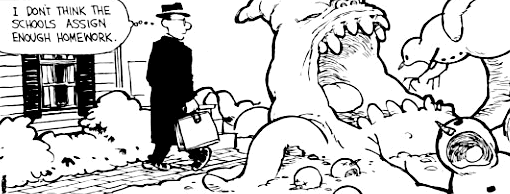
\includegraphics[scale=.4]{figures/schoolmonsters.png}
\end{block}

\end{frame}

\begin{frame}[fragile]
\frametitle{Ambiguity Kills (your parser)}
{\em natural language learning course} \\
(run demos/parsing-ambiguity.py)
\begin{verbatim}
((natural language) (learning course))
(((natural language) learning) course)
((natural (language learning)) course)
(natural (language (learning course)))
(natural ((language learning) course))
\end{verbatim}
\begin{itemize}
\item Some difficult issues:
\begin{itemize}
\item Which one is more plausible?
\item How many analyses for a given input? 
\item Computational complexity of parsing language
\end{itemize}
\end{itemize}
\end{frame}

\begin{frame}
\frametitle{Treebanks}
\begin{itemize}
\item What is the CFG that can be extracted from this single tree: 
\begin{tabbing}
0123\=4567\=8901\=2345\=6789\=0123\=4567 \kill
(S \>(NP (Det the) (NP man)) \\
\> (VP \> (VP \> (V played) \\
\> \> \> (NP (Det a) (NP game))) \\
\> \> (PP \>(P with) \\
\> \> \> (NP (Det the) (NP dog)))))
\end{tabbing}
\end{itemize}
\end{frame}

\begin{frame}
\frametitle{PCFG}
{\small
\[
\begin{array}{cccc}
 S & \rightarrow & NP~VP  & c=1  \\
 NP & \rightarrow & Det~NP & c=3  \\
 NP & \rightarrow & man  & c=1   \\
 NP & \rightarrow & game  & c=1   \\
 NP & \rightarrow & dog  & c=1   \\
 VP & \rightarrow & VP~PP  & c=1  \\
 VP & \rightarrow & V~NP  & c=1  \\
 PP & \rightarrow & P~NP  & c=1  \\
 Det & \rightarrow & the  & c=2  \\
 Det & \rightarrow & a  & c=1   \\
 V & \rightarrow & played & c=1  \\
 P & \rightarrow & with & c=1 
\end{array}
\] 
}
\begin{itemize}
\item We can do this with multiple trees. Simply count occurrences of CFG rules over all the trees. 
\item A repository of such trees labelled by a human is called a TreeBank.
\end{itemize}
\end{frame}

\begin{frame}
\frametitle{Ambiguity}
\begin{itemize}
  \item Part of Speech ambiguity\\
        {\tt saw} $\rightarrow$ {\color{red}noun}\\
        {\tt saw} $\rightarrow$ {\color{red}verb}
  \item Structural ambiguity: Prepositional Phrases\\
        {\tt I saw (the man) with the telescope}\\
        {\tt I saw (the man with the telescope)}
  \item Structural ambiguity: Coordination\\
        {\tt a program to promote safety in ((trucks) and (minivans))}\\
        {\tt a program to promote ((safety in trucks) and (minivans))}\\
        {\tt ((a program to promote safety in trucks) and (minivans))}
\end{itemize}

\end{frame}

\begin{frame}[fragile]
\frametitle{Ambiguity $\leftarrow$ attachment choice in alternative parses}
\includegraphics[scale=.6]{figures/figures.18}
\end{frame}

\begin{frame}
\frametitle{Ambiguity in Prepositional Phrases}
\begin{itemize}
\item<1-> noun attach: {\em I bought the shirt with pockets}
\item<2-> verb attach: {\em I washed the shirt with soap}
\item<3-> As in the case of other attachment decisions in parsing: it depends on the meaning of the entire sentence -- needs world knowledge, etc.
\item<4-> Maybe there is a simpler solution: we can attempt to solve it using heuristics or associations between words
\end{itemize}

\end{frame}

\begin{frame}
\frametitle{Structure Based Ambiguity Resolution}
\begin{itemize}
  \item Right association: a constituent (NP or PP) tends to attach to
  another constituent immediately to its right (Kimball 1973)
  \item Minimal attachment: a constituent tends to attach to an
  existing non-terminal using the fewest additional syntactic nodes
  (Frazier 1978)
  \item These two principles make opposite predictions for
  prepositional phrase attachment
  \item Consider the grammar:
\begin{eqnarray}
VP &\rightarrow& V\ NP\ PP \label{rule:VP}\\
NP &\rightarrow& NP\ PP \label{rule:NP}
\end{eqnarray}  
  for input: {\em I [$_{VP}$ saw [$_{NP}$ the man $\ldots$ [$_{PP}$ with
  the telescope ]}, \\
  RA predicts that the PP attaches to the NP, i.e. use rule (\ref{rule:NP}), \\
  and MA predicts V attachment, i.e. use rule (\ref{rule:VP})
\end{itemize}

\end{frame}

\begin{frame}
\frametitle{Structure Based Ambiguity Resolution}
\begin{itemize}
  \item Garden-paths look structural:\\
  {\rm\it The emergency crews hate most is
  domestic violence}
  \item Neither MA or RA account for more than 55\% of the cases in
  real text 
  \item Psycholinguistic experiments using eyetracking show that humans resolve
  ambiguities as soon as possible in the left to right sequence using
  the words to disambiguate
  \item Garden-paths are caused by a combination of lexical and structural effects:\\ 
  {\rm\it The flowers delivered for the patient arrived}
\end{itemize}

\end{frame}

\begin{frame}
\frametitle{Ambiguity Resolution: Prepositional Phrases in English}
  \begin{itemize}
  \item Learning Prepositional Phrase Attachment: Annotated Data
\begin{tabular}{|cccc|c|}
\hline
v    &     n1   &      p & n2 &       Attachment\\
\hline
join   &   board    &   as &  director & V \\
is       & chairman  &  of  & N.V.    & N \\
using  &   crocidolite & in  & filters & V \\
bring  &   attention  & to  & problem &  V \\ 
is      &  asbestos   & in &  products & N \\
making &   paper    &   for & filters & N \\
including & three     &  with & cancer &  N \\
$\vdots$ & $\vdots$ & $\vdots$ & $\vdots$ & $\vdots$ \\
\hline
\end{tabular}
  \end{itemize}

\end{frame}

\begin{frame}
\frametitle{Prepositional Phrase Attachment}
\begin{tabular}{|l|c|}  \hline
Method & Accuracy \\ \hline
Always noun attachment & 59.0 \\
Most likely for each preposition & 72.2 \\
Average Human (4 head words only) & 88.2 \\
Average Human (whole sentence) & 93.2 \\  \hline
\end{tabular}
\end{frame}

\begin{frame}
\frametitle{Some other studies}
  \begin{itemize}
%    \item {\bf Brill and Resnik, 1994}: \\
%use transformation based learning for PP attachment\\
%80.8\% with words; with Wordnet classes: 81.8\%
  \item {\bf Toutanova, Manning, and Ng, 2004}: 87.54\% using some external knowledge (word classes)
  \item {\bf Merlo, Crocker and Berthouzoz, 1997}: test on multiple PPs
  \begin{itemize}
	\item generalize disambiguation of 1 PP to 2-3 PPs
	\item 14 structures possible for 3PPs assuming a single verb
	\item all 14 are attested in the Penn WSJ Treebank
	\item 1PP: 84.3\% \ \ 2PP: 69.6\% \ \ 3PP: 43.6\% 
  \end{itemize}
  \item {\bf Belinkov+ TACL 2014}: Neural networks for PP attachment (multiple candidate heads)
  \begin{itemize}
	\item NN model (no extra data): 86.6\%
	\item NN model (lots of raw data for word vectors): 88.7\%
	\item NN model with parser and lots of raw data: 90.1\%
  \end{itemize}
  \item {\bf This experiment is still only part of the real problem faced in parsing English}. Plus other sources of ambiguity in other languages
  \end{itemize}


\end{frame}

\lecture{Context Free Grammars}{}
\section{Context Free Grammars}

\begin{frame}
\frametitle{Context-Free Grammars}
\begin{itemize}
\item A CFG is a 4-tuple: $(N, T, R, S)$, where 
\begin{itemize}
\item $N$ is a set of non-terminal symbols, 
\item $T$ is a set of terminal symbols which can include the empty
  string $\epsilon$. $T$ is analogous to $\Sigma$ the alphabet in FSAs.
\item $R$ is a set of rules of the form $A \rightarrow \alpha$, where $A \in N$ and $\alpha \in \{ N \cup T \}^\ast$
\item $S$ is a set of start symbols, $S \in N$
\end{itemize}
\end{itemize}

\end{frame}

\begin{frame}
\frametitle{Context-Free Grammars}
\begin{itemize}
\item Here's an example of a CFG, let's call this one $G$:
\begin{enumerate}
\item $S \rightarrow a\ S\ b$
\item $S \rightarrow \epsilon$
\end{enumerate}
\item What is the language of this grammar, which we will call $L(G)$, the set of strings {\em generated} by this grammar {\color{red} How?} \\
Notice that there cannot be any FSA that corresponds exactly to this set of strings $L(G)$ {\color{red} Why?}
\item What is the {\em tree set} or derivations produced by this grammar?
\end{itemize}

\end{frame}

\begin{frame}
\frametitle{Context-Free Grammars}
\begin{itemize}
\item This notion of generating both the strings and the trees is an important one for Computational Linguistics
\item Consider the trees for the grammar $G'$: $P = \{S~\rightarrow~A~A, A~\rightarrow~a A, A~\rightarrow~A~b, A~\rightarrow~\epsilon \}, $\\
$\Sigma = \{a,b\}, N = \{S,A\}, T = \{a,b,\epsilon\}, S=\{S\}$

\item Why is it called {\em context-free} grammar?
\end{itemize}

\end{frame}

\begin{frame}
\frametitle{Context-Free Grammars}
\begin{itemize}
\item Can the grammar $G'$ produce only trees with equal height subtrees on the left and right? \\
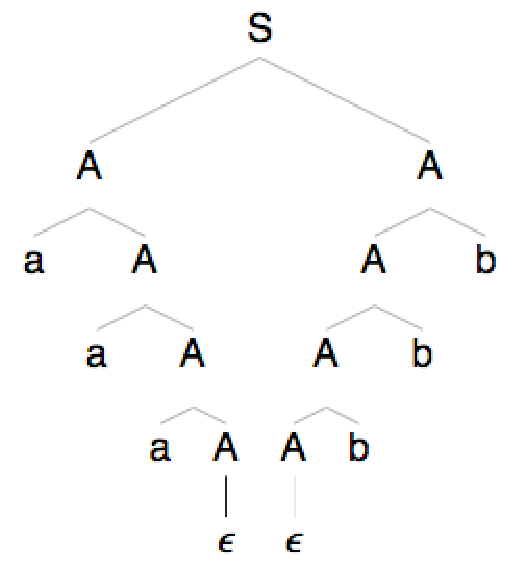
\includegraphics[scale=0.5]{figures/cfg1}
%\Tree [.S [.A a [.A a [.A a [.A $\epsilon$ ] ] ] ] [.A [.A [.A [.A $\epsilon$ ] b ] b ] b ] ]
\end{itemize}

\end{frame}

\begin{frame}
\frametitle{Parse Trees}
\par\noindent
Consider the grammar with rules: 
\begin{eqnarray}
S &\rightarrow& \textit{NP}\ \textit{VP} \nonumber \\
\textit{NP} &\rightarrow& \textit{PRP} \nonumber \\
\textit{NP} &\rightarrow& \textit{DT}\ \textit{NPB} \nonumber \\
\textit{VP} &\rightarrow& \textit{VBP}\ \textit{NP} \nonumber \\
\textit{NPB} &\rightarrow& \textit{NN}\ \textit{NN} \nonumber \\
\textit{PRP} &\rightarrow& \textit{I} \nonumber \\
\textit{VBP} &\rightarrow& \textit{prefer} \nonumber \\
\textit{DT} &\rightarrow& \textit{a} \nonumber \\
\textit{NN} &\rightarrow& \textit{morning} \nonumber \\
\textit{NN} &\rightarrow& \textit{flight} \nonumber
\end{eqnarray}

\end{frame}

\begin{frame}
\frametitle{Parse Trees}

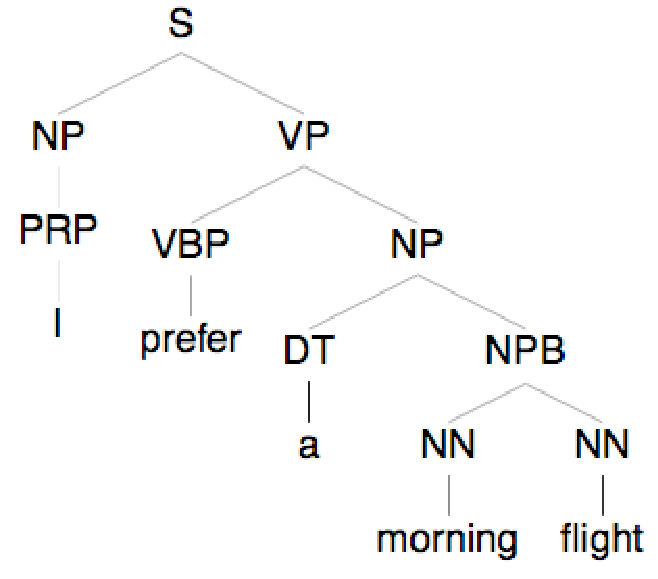
\includegraphics[scale=.5]{figures/cfg2}
%\Tree [.S [.NP [.PRP I ] ] [.VP [.VBP prefer ] [.NP [.DT a ] [.NPB [.NN morning ] [.NN flight ] ] ] ] ]

\end{frame}

\begin{frame}
\frametitle{Parse Trees: Equivalent Representations}
\begin{itemize}
\item (S (NP (PRP I) ) (VP (VBP prefer) (NP (DT a) (NPB (NN morning) (NN flight)))))
\item $[_{S}$ $[_{NP}$ $[_{PRP}$ I ] ] $[_{VP}$ $[_{VBP}$ prefer ]
$[_{NP}$ $[_{DT}$ a ] $[_{NPB}$ $[_{NN}$ morning ] $[_{NN}$ flight ] ] ] ] ]
\end{itemize}

\end{frame}

\begin{frame}
\frametitle{Ambiguous Grammars}
\begin{itemize}
\item $S \rightarrow S\ S$
\item $S \rightarrow a$
\item Given the above rules, consider the input {\em aaa}, what are the valid parse trees?
\item Now consider the input {\em aaaa}
\end{itemize}

\end{frame}

\lecture{Probabilistic Context Free Grammars}{}
\section{Probabilistic Context Free Grammars}

\begin{frame}[fragile]
\frametitle{Probabilistic CFG (PCFG)}
\[
\begin{array}{cccc}
 S & \rightarrow & NP~VP  & 1 \\
 VP & \rightarrow & V~NP  & 0.9 \\
 VP & \rightarrow & VP~PP & 0.1 \\
 PP & \rightarrow & P~NP  & 1 \\
 NP & \rightarrow & NP~PP & 0.25 \\
 NP & \rightarrow & Calvin  & 0.25 \\
 NP & \rightarrow & monsters & 0.25 \\
 NP & \rightarrow & school & 0.25 \\
 V & \rightarrow & imagined  &  1 \\
 P & \rightarrow & in     & 1
\end{array}
\]
\begin{eqnarray}
&P(\textit{input}) = \sum_{\textit{tree}} P(\textit{tree} \mid \textit{input}) \nonumber\\
&P(\textit{Calvin imagined monsters in school}) = ? \nonumber\\
&\textrm{Notice that } P(VP \rightarrow V~NP) + P(VP \rightarrow VP~PP) = 1.0 \nonumber
\end{eqnarray}
\end{frame}

\begin{frame}[fragile]
\frametitle{Probabilistic CFG (PCFG)}
\[ P(\textit{Calvin imagined monsters in school}) = ? \]
\begin{verbatim}
(S (NP Calvin)
   (VP (V imagined)
       (NP (NP monsters)
           (PP (P in)
               (NP school)))))

(S (NP Calvin)
   (VP (VP (V imagined)
           (NP monsters))
       (PP (P in)
           (NP school))))
\end{verbatim}

\end{frame}

\begin{frame}[fragile]
\frametitle{Probabilistic CFG (PCFG)}
\begin{verbatim}
(S (NP Calvin)
   (VP (V imagined)
       (NP (NP monsters)
           (PP (P in)
               (NP school)))))
\end{verbatim}
{\small
\begin{eqnarray*}
P(\textit{tree$_1$})& = & P(S \rightarrow NP\ VP) \times
      P(NP \rightarrow Calvin) \times
      {\color{red} P(VP \rightarrow V\ NP)} \times \nonumber \\
&& P(V \rightarrow imagined) \times 
   {\color{blue} P(NP \rightarrow NP\ PP)} \times
   P(NP \rightarrow monsters) \times \nonumber \\
&& P(PP \rightarrow P\ NP) \times  
   P(P \rightarrow in) \times  
   P(NP \rightarrow school) \nonumber \\
& = & 1 \times 0.25 \times {\color{red} 0.9} \times 1 \times {\color{blue} 0.25} \times 0.25 \times 1 \times 1 \times 0.25 = .003515625 \nonumber 
\end{eqnarray*}
}
\end{frame}

\begin{frame}[fragile]
\frametitle{Probabilistic CFG (PCFG)}
\begin{verbatim}
(S (NP Calvin)
   (VP (VP (V imagined)
           (NP monsters))
       (PP (P in)
           (NP school))))
\end{verbatim}
{\small
\begin{eqnarray*}
P(\textit{tree$_2$})& = & P(S \rightarrow NP\ VP) \times
      P(NP \rightarrow Calvin) \times
      {\color{blue} P(VP \rightarrow VP\ PP)} \times \nonumber \\
&& {\color{red} P(VP \rightarrow V\ NP)} \times
   P(V \rightarrow imagined) \times 
   P(NP \rightarrow monsters) \times \nonumber \\
&& P(PP \rightarrow P\ NP) \times  
   P(P \rightarrow in) \times  
   P(NP \rightarrow school) \nonumber \\
& = & 1 \times 0.25 \times {\color{blue} 0.1} \times {\color{red} 0.9} \times 1 \times 0.25 \times 1 \times 1 \times 0.25 = .00140625 \nonumber 
\end{eqnarray*}
}
\end{frame}

\begin{frame}[fragile]
\frametitle{Probabilistic CFG (PCFG)}
\begin{eqnarray}
P(\textit{Calvin imagined monsters in school}) & = &
P(\textit{tree$_1$}) + P(\textit{tree$_2$}) \nonumber\\ 
& = & .003515625 + .00140625 \nonumber \\
& = & .004921875 \nonumber\\
\textrm{Most likely tree is \textit{tree$_1$}} & = & \argmax{\textit{tree}} P(\textit{tree} \mid \textit{input}) \nonumber
\end{eqnarray}
\bigskip
\begin{minipage}{4in}
\begin{verbatim}
(S (NP Calvin)
   (VP (V imagined)
       (NP (NP monsters)
           (PP (P in)
               (NP school)))))
\end{verbatim}
\end{minipage}
\begin{minipage}{4in}
\begin{verbatim}
(S (NP Calvin)
   (VP (VP (V imagined)
           (NP monsters))
       (PP (P in)
           (NP school))))
\end{verbatim}
\end{minipage}

\end{frame}

\begin{frame}
\frametitle{Probabilistic Context-Free Grammars (PCFG)}
\begin{itemize}
\item A PCFG is a 4-tuple: $(N, T, R, S)$, where 
\begin{itemize}
\item $N$ is a set of non-terminal symbols, 
\item $T$ is a set of terminal symbols which can include the empty
  string $\epsilon$. $T$ is analogous to $\Sigma$ the alphabet in FSAs.
\item $R$ is a set of rules of the form $A \rightarrow \alpha$, where $A \in N$ and $\alpha \in \{ N \cup T \}^\ast$
\item $P(R)$ is the probability of rule $R: A \rightarrow \alpha$ such that $\sum_\alpha P(A \rightarrow \alpha) = 1.0$
\item $S$ is a set of start symbols, $S \in N$
\end{itemize}
\end{itemize}

\end{frame}

\begin{frame}
\frametitle{PCFG}
\begin{itemize}
\item Central condition: \( \sum_\alpha P( A \rightarrow \alpha) = 1 \)
\item Called a {\em proper} PCFG if this condition holds
\item Note that this means $P( A \rightarrow \alpha) = P( \alpha \mid A) = \frac{f(A, \alpha)}{f(A)}$
\item \( P(T \mid S) = \frac{P(T,S)}{P(S)} = P(T,S) = \prod_i P(RHS_i \mid LHS_i) \)
\end{itemize}

\end{frame}



\begin{frame}
\frametitle{PCFG}
\begin{itemize}
\item What is the PCFG that can be extracted from this single tree: 
\begin{tabbing}
0123\=4567\=8901\=2345\=6789\=0123\=4567 \kill
(S \>(NP (Det the) (NP man)) \\
\> (VP \> (VP \> (V played) \\
\> \> \> (NP (Det a) (NP game))) \\
\> \> (PP \>(P with) \\
\> \> \> (NP (Det the) (NP dog)))))
\end{tabbing}
\item How many different rhs $\alpha$ exist for $A \rightarrow \alpha$ where $A$ can be {\it S, NP, VP, PP, Det, N, V, P}
\end{itemize}

\end{frame}

\begin{frame}
\frametitle{PCFG}
{\small
\[
\begin{array}{ccccll}
 S & \rightarrow & NP~VP  & c=1 & p = 1/1 & = 1.0 \\
 NP & \rightarrow & Det~NP & c=3 & p = 3/6 & = 0.5 \\
 NP & \rightarrow & man  & c=1 & p = 1/6 & = 0.1667 \\
 NP & \rightarrow & game  & c=1 & p = 1/6 & = 0.1667 \\
 NP & \rightarrow & dog  & c=1 & p = 1/6 & = 0.1667 \\
 VP & \rightarrow & VP~PP  & c=1 & p = 1/2 & = 0.5 \\
 VP & \rightarrow & V~NP  & c=1 & p = 1/2 & = 0.5 \\
 PP & \rightarrow & P~NP  & c=1 & p = 1/1 & = 1.0 \\
 Det & \rightarrow & the  & c=2 & p = 2/3 & = 0.67 \\
 Det & \rightarrow & a  & c=1 & p = 1/3 & = 0.33 \\
 V & \rightarrow & played & c=1 & p = 1/1 & = 1.0 \\
 P & \rightarrow & with & c=1 & p = 1/1 & = 1.0 \\
\end{array}
\] 
}
\begin{itemize}
\item We can do this with multiple trees. Simply count occurrences of CFG rules over all the trees. 
\item A repository of such trees labelled by a human is called a TreeBank.
\end{itemize}
\end{frame}


%\begin{frame}
%\frametitle{Parsing PCFGs: CKY algorithm $+$ Viterbi}
%{\small\begin{frame}
%$p: S \rightarrow S\ S\ ,\ 1-p: S \rightarrow a$
%\end{frame}}
%\begin{frame}
%\begin{tabular}{|c|c|c|c|}
%\hline
% a & a & a & a \\
%\hline
%$1-p$: S$_{0,1}$ $\rightarrow$ a & $1-p$: S$_{1,2}$ $\rightarrow$ a & $1-p$: S$_{2,3}$ $\rightarrow$ a & $1-p$: S$_{3,4}$ $\rightarrow$ a \\
%\hline
% S$_{0,1}$ $+$  S$_{1,2}$ & S$_{1,2}$ $+$  S$_{2,3}$ & S$_{2,3}$ $+$  S$_{3,4}$ & \\
% $=$ S$_{0,2}$ $\rightarrow$ S\ S & $=$ S$_{1,3}$ $\rightarrow$ S\ S & $=$ S$_{2,4}$ $\rightarrow$ S\ S & \\
% $p(1-p)^2$ & $p(1-p)^2$  & $p(1-p)^2$  & \\
%\hline
% S$_{0,1}$ $+$  S$_{1,3}$ & S$_{1,2}$ $+$  S$_{2,4}$ & & \\
% OR & OR & & \\
% S$_{0,2}$ $+$  S$_{2,3}$ &   S$_{1,3}$ $+$  S$_{3,4}$ & & \\
% $=$ S$_{0,3}$ $\rightarrow$ S\ S &  $=$ S$_{1,4}$ $\rightarrow$ S\ S & &\\
%$\textrm{max}(p^2(1-p)^3,$ & $\textrm{max}(p^2(1-p)^3,$ & & \\
%$p^2(1-p)^3)$ & $p^2(1-p)^3)$ & & \\
%\hline
% {\em What goes in this cell?} & & & \\
% ?? $=$ S$_{0,4}$ &&& \\
%\hline
%\end{tabular}
%\end{frame}
%
%\end{frame}

%\begin{frame}
%\frametitle{Example PCFG}
%\[
%\begin{array}{cccc}
% S & \rightarrow & NP~VP  & 1 \\
% VP & \rightarrow & V~NP  & 0.9 \\
% VP & \rightarrow & VP~PP & 0.1 \\
% PP & \rightarrow & P~NP  & 1 \\
% NP & \rightarrow & NP~PP & 0.25 \\
% NP & \rightarrow & Calvin  & 0.25 \\
% NP & \rightarrow & monsters & 0.25 \\
% NP & \rightarrow & school & 0.25 \\
% V & \rightarrow & imagined  &  1 \\
% P & \rightarrow & in     & 1
%\end{array}
%\] 
%
%\end{frame}

%\begin{frame}
%\frametitle{CKY Viterbi}
%\begin{frame}
%\begin{tabular}{|c|c|c|c|c|}
%\hline
% Calvin & imagined & monsters & in & school \\
%\hline
% NP$_{0,1}$ & V$_{1,2}$  &NP$_{2,3}$ &  P$_{3,4}$ &  NP$_{4,5}$ \\
%$0.25$ & $1$ & $0.25$ & $1$ & $0.25$ \\
%\hline
% & V$_{1,2}$ $+$  NP$_{2,3}$ & & P$_{3,4}$ $+$ NP$_{4,5}$ &\\
% & $=$ VP$_{1,3}$ $\rightarrow$ V\ NP & & $=$ PP$_{3,5}$ $\rightarrow$ P NP & \\
% & $1 \times 0.25 \times 0.9$  &  & $1^2 \times 0.25$ & \\
%\hline
%  &  VP$_{1,3}$ $+$ PP$_{3,5}$ & NP$_{2,3}$ $+$ PP$_{3,5}$ & & \\
% &   OR & $=$ NP$_{2,5}$ $\rightarrow$ NP PP  & &\\
% &   V$_{1,2}$ $+$ NP$_{2,5}$ & $0.25^3$  & &\\
%  &  $=$ VP$_{1,5}$   & & & \\
% & $x$ & &&\\
%\hline
% & && & \\
% $=$ S$_{0,4}$ &&& &\\
% $x \times 0.25$ &&& &\\
%\hline
%\end{tabular}
%\end{frame}
%
%\end{frame}

\begin{frame}
\frametitle{Ambiguity}
\begin{itemize}
  \item Part of Speech ambiguity\\
        {\tt saw} $\rightarrow$ {\color{red}noun}\\
        {\tt saw} $\rightarrow$ {\color{red}verb}
  \item Structural ambiguity: Prepositional Phrases\\
        {\tt I saw (the man) with the telescope}\\
        {\tt I saw (the man with the telescope)}
  \item Structural ambiguity: Coordination\\
        {\tt a program to promote safety in ((trucks) and (minivans))}\\
        {\tt a program to promote ((safety in trucks) and (minivans))}\\
        {\tt ((a program to promote safety in trucks) and (minivans))}
\end{itemize}

\end{frame}

\begin{frame}[fragile]
\frametitle{Ambiguity $\leftarrow$ attachment choice in alternative parses}
\includegraphics[scale=.6]{figures/figures.18}
\end{frame}

\begin{frame}
\frametitle{Parsing as a machine learning problem}
\begin{itemize}
\item<1-> $S = $ a sentence \\
      $T = $ a parse tree \\
A statistical parsing model defines $P(T \mid S)$
\item<2-> Find best parse: $\textrm{arg max}\atop{T}$ $P(T \mid S)$
\item<3-> $P(T \mid S) = \frac{P(T, S)}{P(S)} = P(T,S)$
\item<4-> Best parse: $\textrm{arg max}\atop{T}$ $P(T, S)$
\item<5-> e.g. for PCFGs: $P(T, S) = \prod_{i=1 \ldots n} P(\textrm{RHS}_i \mid \textrm{LHS}_i)$
\end{itemize}

\end{frame}

\newcommand{\code}[1]{\mbox{\tt #1}}

\begin{frame}
\frametitle{Adding Lexical Information to PCFG}
\centering
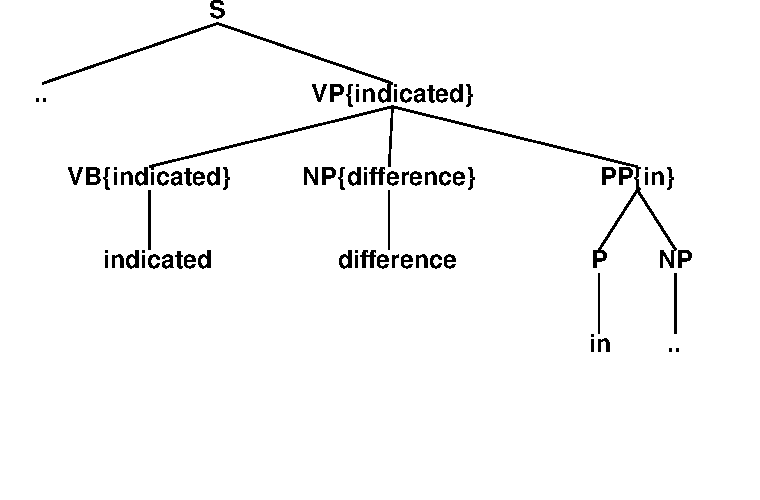
\includegraphics[scale=.7]{figures/bilexicalcfg0}
\end{frame}

\begin{frame}
\frametitle{Adding Lexical Information to PCFG {\footnotesize (Collins 99, Charniak 00)}}
\begin{center}
  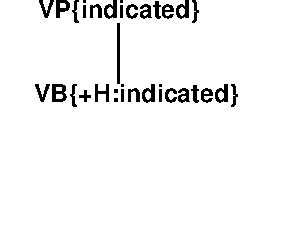
\includegraphics[scale=.5]{figures/bilexicalcfg1} \ 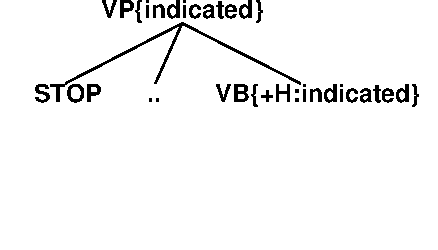
\includegraphics[scale=.5]{figures/bilexicalcfg2} \ 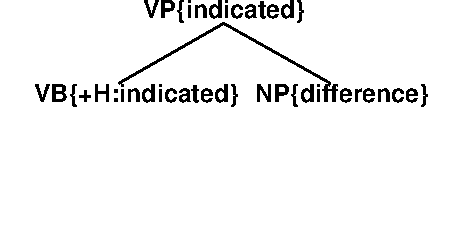
\includegraphics[scale=.5]{figures/bilexicalcfg3} 
\\ 
 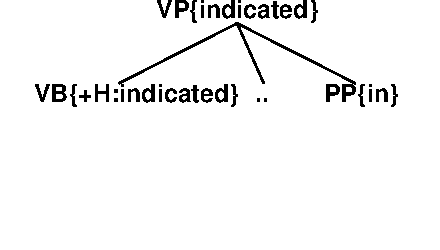
\includegraphics[scale=.5]{figures/bilexicalcfg4} \
 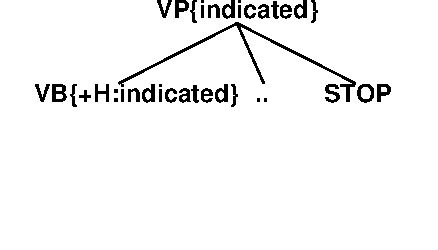
\includegraphics[scale=.5]{figures/bilexicalcfg5} 
\[ \begin{array}{l}
 P_h(\code{VB} \mid \code{VP}, \code{indicated}) \times 
 P_l(\code{STOP} \mid \code{VP}, \code{VB}, \code{indicated}) \times
 \\ 
 P_r(\code{NP(difference)} \mid \code{VP}, \code{VB},
 \code{indicated}) \times \\
 P_r(\code{PP(in)} \mid \code{VP}, \code{VB}, \code{indicated}) \times
 \\ 
 P_r(\code{STOP} \mid \code{VP}, \code{VB}, \code{indicated})
 \end{array} \]
\end{center}
\end{frame}

%\begin{frame}
%\frametitle{Adding Additional Features to PCFGs {\footnotesize (Collins 99)}}
%  \begin{center}
%  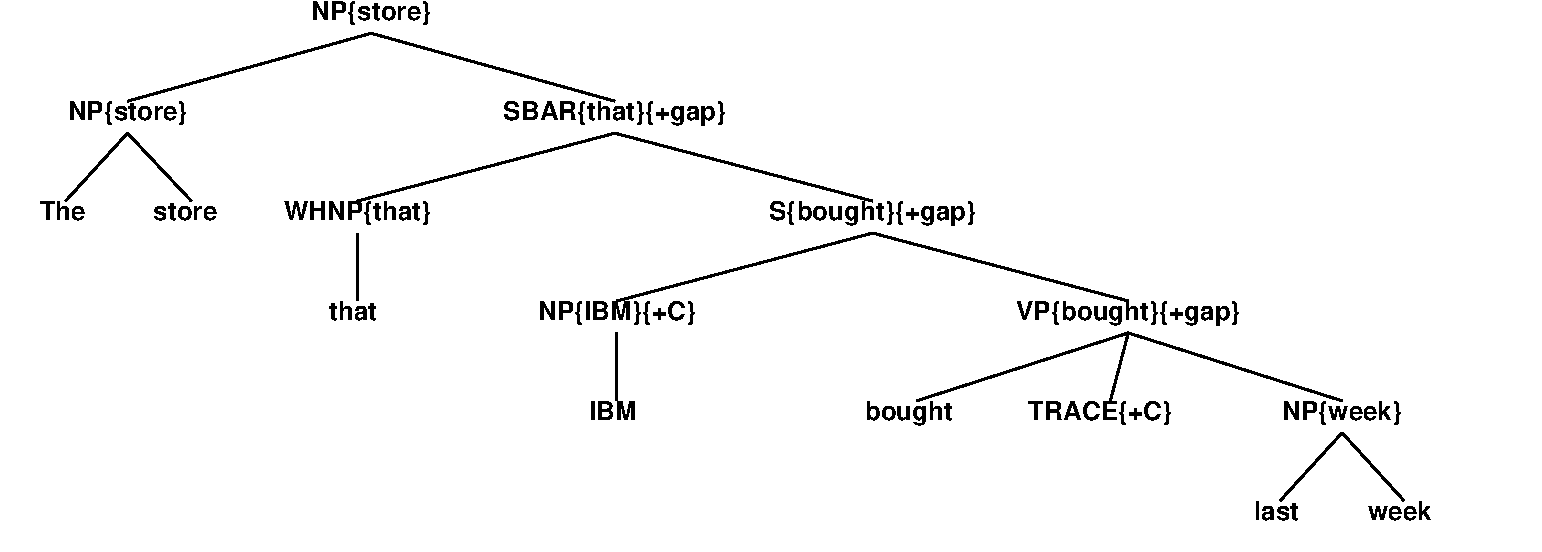
\includegraphics[scale=.4]{figures/cfgfeat}
%  \end{center}
%  {\footnotesize\tt
%  \begin{tabular}{lllllll}
%  NP           & $\rightarrow$ & [ & NP\{+H\}  & SBAR\{+gap\}          &    & ] \\
%  SBAR\{+gap\} & $\rightarrow$ & [ & WHNP      & S\{+H\}\{+C\}\{+gap\} &    & ] \\
%  S\{+gap\}    & $\rightarrow$ & [ & NP\{+C\}  & SBAR\{+H\}\{+gap\}    &    & ] \\
%  VP\{+gap\}   & $\rightarrow$ & [ & VB\{+H\}  & TRACE\{+C\}           & NP & ]
%  \end{tabular}}
%\end{frame}

\begin{frame}[fragile]
\frametitle{Evaluation of Parsing}
\begin{itemize}
\item Consider a candidate parse to be evaluated against the truth (or gold-standard parse):
{\footnotesize
\begin{verbatim}
candidate: (S (A (P this) (Q is)) (A (R a) (T test)))
gold:      (S (A (P this)) (B (Q is) (A (R a) (T test))))
\end{verbatim}
}
\item In order to evaluate this, we list all the constituents
{\small\begin{center}
\begin{tabular}{|l|l|}
\hline
Candidate & Gold \\
\hline
(0,4,S) & (0,4,S) \\
(0,2,A) & (0,1,A) \\
(2,4,A) & (1,4,B) \\
        & (2,4,A) \\
\hline
\end{tabular}
\end{center}
}
\item Skip spans of length 1 which would be equivalent to part of speech
tagging accuracy.
\item Precision is defined as $\frac{\#correct}{\#proposed} = \frac{2}{3}$
and recall as $\frac{\#correct}{\#in\ gold} = \frac{2}{4}$. 
\item Another measure: crossing brackets,
{\small\begin{verbatim}
candidate: [ an [incredibly expensive] coat ] (1 CB)
gold:      [ an [incredibly [expensive coat]]
\end{verbatim}
}
\end{itemize}
\end{frame}

\begin{frame}[fragile]
\frametitle{Evaluation of Parsing}
{\footnotesize
\[
\begin{array}{lcl}
\mbox{Bracketing recall}\ R & = & \frac{\mbox{num of correct constituents}}{\mbox{num of constituents in the goldfile}} \\
\\
\mbox{Bracketing precision}\ P & = & \frac{\mbox{num of correct constituents}}{\mbox{num of constituents in the parsed file}} \\
\\
\mbox{Complete match} & = & \mbox{\% of sents where recall \& precision are both 100\%} \\
\\
\mbox{Average crossing} & = & \frac{\mbox{num of constituents crossing a goldfile constituent}}{\mbox{num of sents}} \\
\\
\mbox{No crossing} & = & \mbox{\% of sents which have $0$ crossing brackets} \\
\\
\mbox{$2$ or less crossing} & = & \mbox{\% of sents which have $\leq 2$ crossing brackets}
\end{array}
\]
}
\end{frame}

\begin{frame}
\frametitle{Statistical Parsing Results}
\begin{center}
\footnotesize
\[ \textrm{F1-score} = 2 \frac{\textit{precision} \cdot \textit{recall}}{\textit{precision} + \textit{recall}} \]
\begin{tabular}{|p{7cm}|l|}
\hline
  & $\leq 100 wds$  \\
System & F1-score \\
\hline
Shift-Reduce (Magerman, 1995)   & 84.14 \\
PCFG with Lexical Features (Charniak, 1999)   & 89.54 \\
Unlexicalized Berkeley parser (Petrov et al, 2007) & 90.10 \\
$n$-best Re-ranking (Charniak and Johnson, 2005) & 91.02 \\
Tree-insertion grammars (Carreras, Collins, Koo, 2008) & 91.10 \\
Ensemble $n$-best Re-ranking (Johnson and Ural, 2010) & 91.49 \\
Forest Re-ranking (Huang, 2010) & 91.70 \\
Unlabeled Data with Self-Training (McCloskey et al, 2006) & 92.10 \\
\hline
Self-Attention (Kitaev and Klein, 2018) & 93.55 \\
Self-Attention with unlabeled data (Kitaev and Klein, 2018) & 95.13 \\
\hline
\end{tabular}
\end{center}
\end{frame}

\begin{frame}
\frametitle{Practical Issues: Beam Thresholding and Priors}
\begin{itemize}
\item Probability of nonterminal $X$ spanning $j \ldots k$:
$N[X,j,k]$
\item Beam Thresholding compares $N[X,j,k]$ with every other $Y$
where $N[Y,j,k]$
\item But what should be compared?
\item Just the {\em inside probability}: $P(X \stackrel{*}{\Rightarrow} t_j
\ldots t_k)$?\\
written as $\beta(X, j, k)$
\item Perhaps $\beta(\mbox{\tt FRAG}, 0, 3) > \beta(\mbox{\tt NP}, 0,
3)$, but {\tt NP}s are much more likely than {\tt FRAG}s in general
\end{itemize}
\end{frame}

\begin{frame}
\frametitle{Practical Issues: Beam Thresholding and Priors}
\begin{itemize}
\item The correct estimate is the {\em outside probability}: 
\[ P(S \stackrel{*}{\Rightarrow} t_1 \ldots t_{j-1}\ X\ t_{k+1} \ldots
t_n) \]\\
written as $\alpha(X, j, k)$ 
\item Unfortunately, you can only compute $\alpha(X, j, k)$
efficiently after you finish parsing and reach $(S, 0, n)$
\end{itemize}
\end{frame}

\begin{frame}
\frametitle{Practical Issues: Beam Thresholding and Priors}
\begin{itemize}
\item To make things easier we multiply the prior probability $P(X)$
with the inside probability
\item In beam Thresholding we compare every new insertion of $X$ for
span $j, k$ as follows:\\
Compare $P(X) \cdot \beta(X,j,k)$ with the most probable $Y$ $P(Y) \cdot
\beta(Y,j,k)$
\item Assume $Y$ is the most probable entry in $j,k$, then we compare
\begin{eqnarray}
\textsf{beam} \cdot P(Y) \cdot \beta(Y,j,k) \label{eq:1} \\
P(X) \cdot \beta(X,j,k) \label{eq:2}
\end{eqnarray}
\item If $(\ref{eq:2}) < (\ref{eq:1})$ then we prune $X$ for this span $j,k$ 
\item \textsf{beam} is set to a small value, say 0.001 or even 0.01. 
\item As the beam value increases, the parser speed increases (since more entries are pruned).
\item A simpler (but not as effective) alternative to using the beam is to keep only the top $K$ entries for each span $j,k$
%\item Other more sophisticated methods are given in (Goodman 1997)
\end{itemize}
\end{frame}

\begin{frame}
\frametitle{Experiments with Beam Thresholding}
%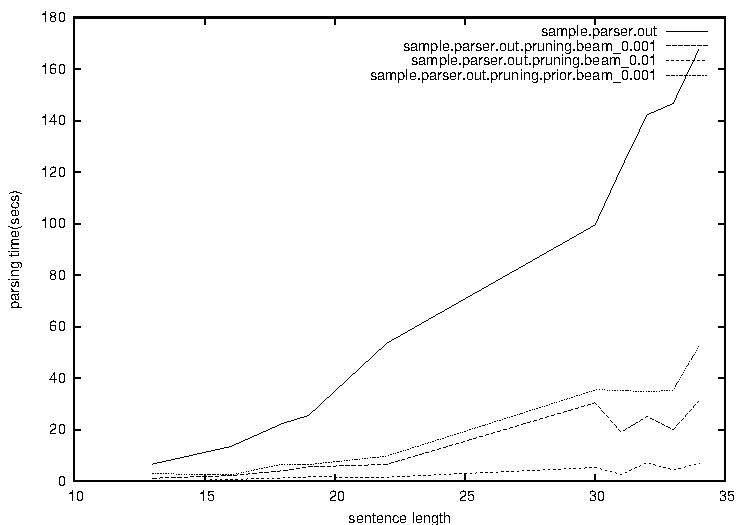
\includegraphics[scale=.85]{figures/parsetimes}
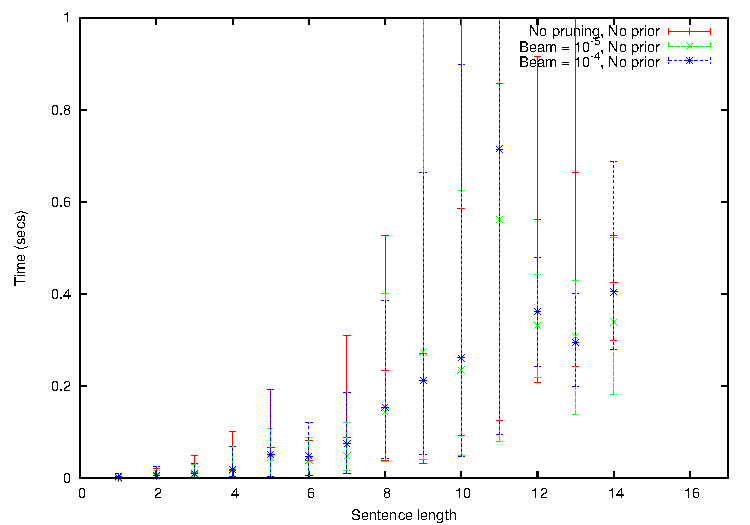
\includegraphics[scale=.85]{figures/timing-without-prior.pdf}
\end{frame}

\begin{frame}
\frametitle{Experiments with Beam Thresholding}
%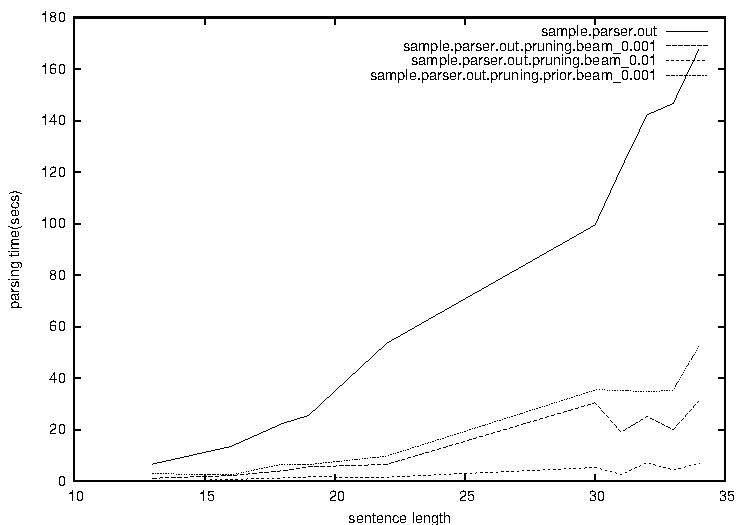
\includegraphics[scale=.85]{figures/parsetimes}
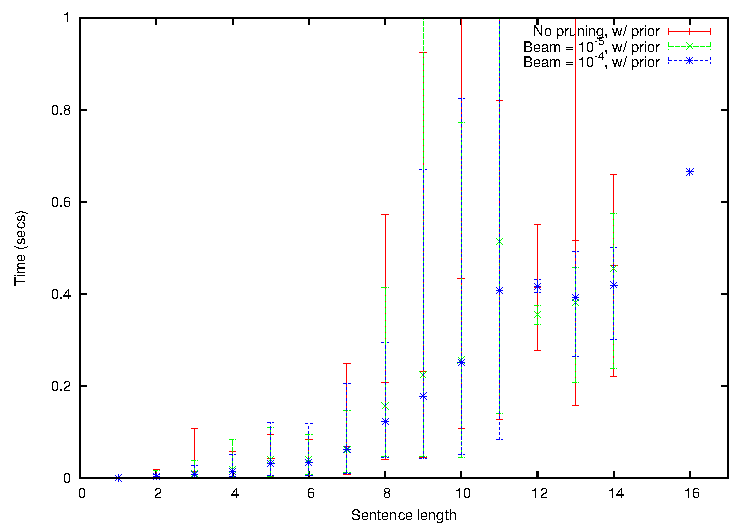
\includegraphics[scale=.85]{figures/timing-with-prior.pdf}
\end{frame}

\end{document}
